\documentclass[a4paper,12pt, oneside]{book}

%\usepackage{fullpage}
\usepackage[italian]{babel}
\usepackage[utf8]{inputenc}
\usepackage{amssymb}
\usepackage{amsthm}
\usepackage{graphics}
\usepackage{amsfonts}
\usepackage{amsmath}
\usepackage{amstext}
\usepackage{engrec}
\usepackage{rotating}
\usepackage{verbatim}
\usepackage[safe,extra]{tipa}
\usepackage{showkeys}
\usepackage{multirow}
\usepackage{hyperref}
\usepackage{microtype}
\usepackage{enumerate}
\usepackage{braket}
\usepackage{marginnote}
\usepackage{pgfplots}
\usepackage{cancel}
\usepackage{polynom}
\usepackage{booktabs}
\usepackage{enumitem}
\usepackage{framed}
\usepackage{pdfpages}
\usepackage{pgfplots}
\usepackage{fancyhdr}
\pagestyle{fancy}
\fancyhead[LE,RO]{\slshape \rightmark}
\fancyhead[LO,RE]{\slshape \leftmark}
\fancyfoot[C]{\thepage}


\title{Fisica}
\author{UniShare\\\\Davide Cozzi\\\href{https://t.me/dlcgold}{@dlcgold}}
\date{}

\pgfplotsset{compat=1.13}
\begin{document}
\maketitle

\definecolor{shadecolor}{gray}{0.80}

\newtheorem{teorema}{Teorema}
\newtheorem{definizione}{Definizione}
\newtheorem{esempio}{Esempio}
\newtheorem{corollario}{Corollario}
\newtheorem{lemma}{Lemma}
\newtheorem{osservazione}{Osservazione}
\newtheorem{nota}{Nota}
\newtheorem{esercizio}{Esercizio}
\tableofcontents

\renewcommand{\chaptermark}[1]{%
\markboth{\chaptername
\ \thechapter.\ #1}{}}
\renewcommand{\sectionmark}[1]{\markright{\thesection.\ #1}}

\chapter{Introduzione}
\textbf{Questi appunti sono presi a lezione. Per quanto sia stata fatta una revisione è altamente probabile (praticamente certo) che possano contenere errori, sia di stampa che di vero e proprio contenuto. Per eventuali proposte di correzione effettuare una pull request. Link: } \url{https://github.com/dlcgold/Appunti}.\\
\textbf{Grazie mille e buono studio!}

\chapter{Meccanica}
Si comincia con la Meccanica, la branca della fisica classica che studia il moto dei corpi, esprimendolo con leggi quantitative. Si ha la seguente divisione:
\begin{itemize}
\item \textbf{Cinematica}, dove si studia il moto e le sue caratteristiche indipendentemente dalle cause
\item \textbf{Dinamica}, dove si studia l'influenza delle forze nel moto 
\end{itemize}
Si utilizzano i cosiddetti \textit{punti materiali} per semplificare lo studio dei fenomeni. Un punto materiale infatti non ha estensione ma è dotato di una massa. In pratica ha dimensioni trascurabili rispetto allo spazio nel quale si muove.\\
Un altro strumento essenziale per lo studio dei fenomeni è il \textit{sistema di riferimento} mediante gli assi ortogonali:
\begin{center}
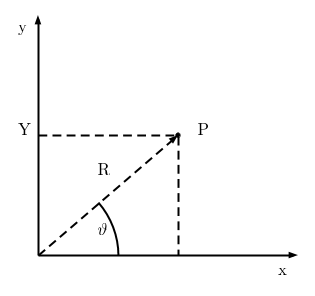
\includegraphics[scale=0.7]{img/ref.png}
\end{center}
\newpage
e si hanno le seguenti formule:
$$R=\sqrt{X^2+Y^2}$$
$$sin \vartheta=\frac{Y}{R}$$
$$cos \vartheta=\frac{X}{R}$$
$$tan \vartheta = \frac{Y}{X}$$
$$\vartheta= arctan \frac{Y}{X}$$
e per gli angoli si usano i \textit{radianti} in quanto adimensionali. L'angolo in radianti infatti è:
$$\vartheta_{rad}=\frac{Lunghezza\_arco}{raggio}$$
dove le due unità di misura esprimenti una lunghezza vengono "semplificate".\\
Si ricordano inoltre le basi del calcolo vettoriale. Tra due vettori posso fare somme e sottrazioni 
La somma non è altro che la diagonale maggiore del parallelogramma che si forma tra i due vettori. Inoltre se $\vec{A}=(a_x,a_y)$ e $\vec{B}=(b_x,b_y)$ si ha:
$$\vec{C}=\vec{A}+\vec{B}=(a_x+b_x, a_y+b_y)$$
la sottrazione è la diagonale minore e:
$$\vec{C}=\vec{A}-\vec{B}=(a_x-b_x, a_y-b_y)$$
\begin{center}
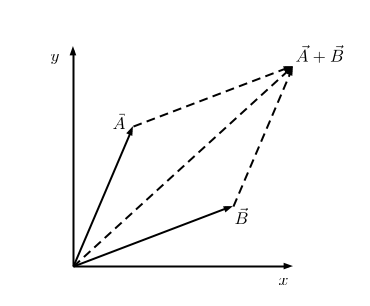
\includegraphics[scale=0.5]{img/vec.png}
\quad
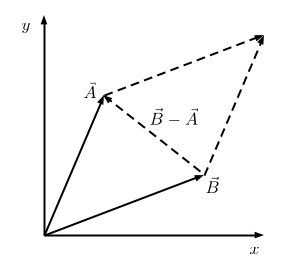
\includegraphics[scale=0.5]{img/vec2.png}
\end{center}
\section{Cinematica}
Innanzitutto qualche definizione:
\begin{itemize}
\item \textbf{Moto:} posizione in funzione del tempo in un dato sistema di riferimento
\item \textbf{Traiettoria:} luogo dei punti attraversati dal punto materiale in movimento
\item \textbf{Velocità:} variazione della posizione
\item \textbf{Accelerazione:} variazione della velocità
\item \textbf{Quiete:} assenza di movimento in un certo sistema di riferimento
\end{itemize}
Come grandezze fondamentali del movimento si hanno quindi \textit{posizione}, \textit{velocità} e \textit{accelerazione}, tutte e tre funzioni del tempo.
\subsection{Moto Rettilineo}
Rappresentando su un piano cartesiano avente la posizione come ordinata e il tempo come ascisse e rappresentando vri momenti del moto si ottiene una curva. Questa curva rappresenta la legge oraria.\\
Si ha la traiettoria più semplice, una retta. Il moto del punto quindi è esprimibile come funzione solo di $$\vec{x}(t)$$, che sarà la nostra equazione del moto.\\
Si passa quindi da un sistema di riferimento a 3 assi:
\begin{center}
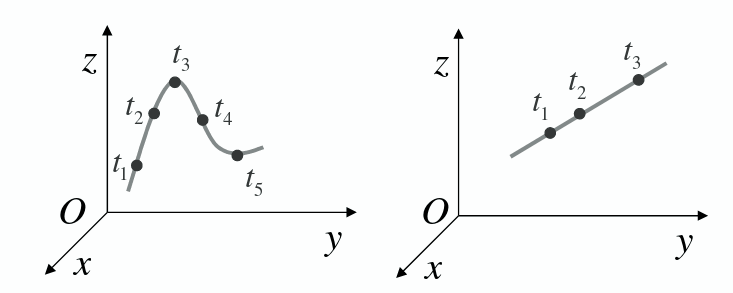
\includegraphics[scale=0.5]{img/rett.png}
\end{center}
ad uno a un asse:
\begin{center}
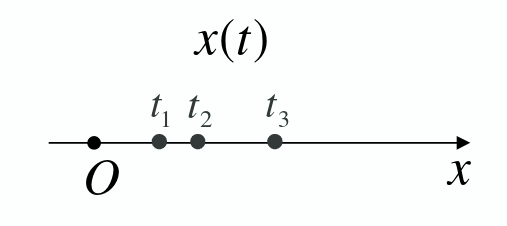
\includegraphics[scale=0.3]{img/ret2.png}
\end{center}
La scelta dell'origine della coordinata spaziale ($x=0$) e di quella temporale ($t=0$) sono arbitrari.\\
Si definisce la \textbf{distanza} come una quantità scalare la lunghezza del tratto percorso da un punto per cambiare posizione.
\subsubsection{Velocità}
Per ottenere la velocità di un punto materiale ne misuro la posizione in due diversi istanti di tempo. Si ha:
\begin{itemize}
\item \textbf{Spostamento:} $\Delta \vec{x}= x(t_2)-x(t_1)=x_2-x_1$ è un vettore che descrive la differenza di posizione tra due punti. Viene misurato in \textit{Metri (m)} secondo il Sistema Internazionale (SI). Il metro è definito come la distanza percorsa dalla luce in $\frac{1}{299792458}s$ 
\item \textbf{Intervallo di Tempo:} $\Delta t=t_2-t_1$ che viene misurato in \textit{Secondi (s)} secondo il Sistema Internazionale (SI). Il secondo è definito come la durata di $9192631770$ periodi della radiazione corrispondente alla transizione tra 2 livelli iperfini dello stato fondamentale dell'atomo di Cesio-133
\end{itemize}
Possiamo quindi definire la \textbf{Velocità Media:}
$$v_m=\frac{\Delta \vec{x}}{\Delta t}=\frac{x_2-x_1}{t_2-t_1}=\frac{\vec{v_2}-\vec{v_1}}{2}$$
Questa grandezza però non fornisce nessuna indicazione sulle caratteristiche effettive del moto. Provo a spezzare il moto in più intervalli temporali al fine di studiarne ogni variazione. Si ottiene quindi la \textbf{Velocità Istantanea}:
$$v=\lim_{\Delta t \to 0}\frac{\Delta \vec{x}}{\Delta t}=\frac{d \vec{x}(t)}{d t}$$
La velocità istantanea rappresenta la rapidità di variazione temporale della posizione nell'istante \textit{t} considerata. Il segno della velocità indica la direzione del moto sull'asse delle ascisse. La velocità è a sua volta funzione del tempo:
$$v(t)=\frac{d\vec{x}(t)}{dt}$$
che è ben rappresentata dai seguenti grafici:
\begin{center}
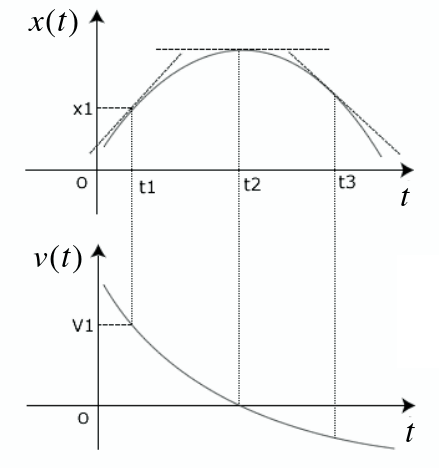
\includegraphics[scale=0.36]{img/ist.png}
\end{center}
Se \textit{v} è costante si parla di \textit{Moto Rettilineo Uniforme}. \\
Si ha quindi:
$$\Delta x = v\Delta t\to x-x_0=v(t-t_0)\to x=x_0+v(t-t_0)$$
che vale anche per $v$ non costante ma per intervalli di tempo approssimati 0, infatti tra brevi istanti di tempo si può approssimare la velocità istantanea $v(t)=\frac{dx}{dt}$ come una velocità costante. Disegniamo ora un grafico velocità tempo con la curva rappresentante la legge oraria, indicando velocità e tempo in due momenti del moto:
\begin{center}
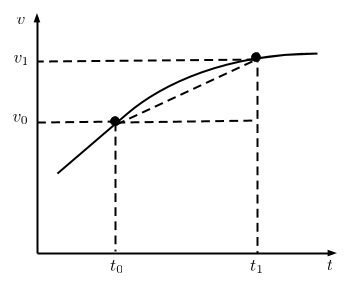
\includegraphics[scale=0.5]{img/gra.png}
\end{center}
calcolare l'area sottesa alla curva implica calcolare la differenza di posizione. Approssimo la curva ad una retta e procedo col banale calcolo del trapezio sottostante:
$$A=(t_1-t_0)(\frac{\vec{v_1}-\vec{v_0}}{2})+(t_1-t_0
)\vec{v_0}=(\frac{\vec{v_1}-\vec{v_0}}{2})\Delta t+\vec{v_0}\Delta t$$
$$A=\frac{\Delta t}{2}(\vec{v_1}-\vec{v_0}+2\vec{v_0})=\frac{\Delta t}{2}(\vec{v_0}+\vec{v_1})=\Delta t v_{med}$$
Nota quindi l'equazione del moto $$\vec{x}(t)$$ possiamo ricavare $v(t)$ derivando, infatti la posizione si ottiene, partendo dal grafico sopra, riducendo al massimo gli intervalli di tempo e calcolando la somma delle aree dei vari rettangolini .\\
Si può procedere anche al calcolo di $$\vec{x}(t)$$ avendo nota $\vec{v}(t)$. Sappiamo che lo spostamento totale è: $\Delta \vec{x}=\sum_{i=1}^n \Delta \vec{x}_i=\sum_{i=1}^n v_{m_i} \Delta t$ e che, per intervalli infinitesimi $dx=\vec{v}(t) dt$. Si ha quindi:
$$\Delta x=\underbrace{\int_{x_0}^x dx}_{\vec{x}(t)-x_0}=\int_{t_0}^t \vec{v}(t) dt$$
$$\downarrow$$
$$\vec{x}(t)=x_0+\int_{t_0}^t \vec{v}(t) dt$$
che è l'equazione del moto rettilineo per una velocità qualunque.\\
Possiamo ora anche riscrivere la forma completa della velocità media, essendo $x-x_0=\int_{t_0}^t \vec{v}(t) dt$ si ha:
$$v_m=\frac{1}{t-t_0}\int_{t_0}^t \vec{v}(t) dt$$
Possiamo analizzare ora il \textit{moto rettilineo uniforme} con \textit{v} costante. Essendo \textit{v} costante, e non più dipendente dal tempo, può essere portata fuori dall'integrale:
$$\vec{x}(t)=x_0+v\int_{t_0}^t dt=x_0+v(t-t_0)$$
che è l'equazione generale del moto rettilineo uniforme dove lo spostamento varia linearmente col tempo.\\
La velocità di esprime in metri al secondo ($\frac{m}{s}$ o \textit{m/s}) o in kilometri all'ora $\frac{km}{h}$ o \textit{km/h}). Per passare da \textit{km/h} a \textit{m/s} divido la grandezza in \textit{km/h} per 3,6, per passare da \textit{m/s} a \textit{km/h} moltiplico la grandezza in \textit{m/s} per 3,6. 
\subsubsection{Accelerazione}
Si ha che in due istanti di tempo diversi abbiamo due diverse velocità: $\vec{v}(t_1)=\vec{v_1}$ e $\vec{v}(t_2)=\vec{v_2}$. Si definisce l'\textbf{Accelerazione Media:}
$$a_m=\frac{\vec{v_2}-\vec{v_1}}{t_2-t_1}=\frac{\Delta v}{\Delta t}$$
Procediamo come per la velocità, con un grafico accelerazione-tempo e la legge del moto, calcolando l'area sottostante ottengo la differenza di posizione. Si ha una situazione più semplice ancora perché avendo $a$ costante (e quindi $ \overline{a}(t)=a_{med}=\frac{\Delta v}{\Delta t}$ e quindi $v_1=v_0+a(t_1-t_0)$) essa può essere rappresentata come una retta l'area sottostante, che questa volta è letteralmente un trapezio senza approssimazioni, è lo spostamento.
\begin{center}
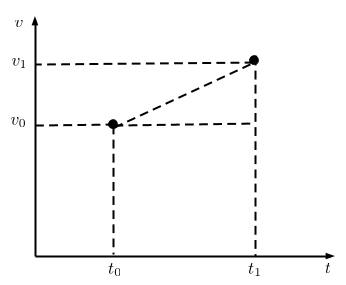
\includegraphics[scale=0.5]{img/gra2.png}
\end{center}
ovvero:
$$A=x-x_0=t_1-v_0+\frac{t_1(v_1-v_0)}{2}=t_1\frac{v_1+v_0}{2}$$ 
e quindi 
$$v_1=v_0+at_1$$
unendo con $v_1=v_0+a(t_1-t_0)$ si ottiene:
$$x-x_0=\frac{t_1}{2}(v_0+at_1+v_0)=\frac{t_1}{2}(2v_0+at_1)=v_0t_1+\frac{a}{2}t_1^2$$
$$\downarrow$$
$$x=x_0+v_0t_1+\frac{a}{2}t_1^2$$
Ora, come per la velocità, analizziamo intervalli di tempo infinitesimi ricordando che anche l'accelerazione è una funzione del tempo:
$$a(t)=\frac{dv}{dt}=\frac{d}{dt}\left(\frac{dx}{dt}\right)=\frac{d^2x}{dt^2}$$
ovvero la derivata seconda della posizione rispetto al tempo e si ha che:
\begin{itemize}
\item $a=0$ implica un moto rettilineo uniforme (si deriva una costante, \textit{v}, e si ottiene 0)
\item $a>0$ implica una velocità crescente
\item $a<0$ implica una velocità decrescente
\end{itemize}
\begin{shaded}
Proviamo ora a risalire a $\vec{v}(t)$ conoscendo \textit{a(t)}. Sappiamo che $a=\frac{dv}{dt}\rightarrow dv=a(t) dt$. Risolviamo quindi l'equazione differenziale :
$$\int_{\vec{v_0}}^v dv = \int_{t_0}^t a(t) dt\rightarrow \vec{v}(t)=\vec{v_0}+\int_{t_0}^t a(t) dt$$
che è l'equazione generale per la velocità, dove, nel caso di $a\neq 0$, ovvero di accelerazione costante, si ha:
$$\vec{v}(t)=\vec{v_0}+a\int_{t_0}^t dt=\vec{v_0}+a (t-t_0)$$
dove si nota come la velocità sia una funzione lineare del tempo se $t_0=0$, ottenendo $\vec{v}(t)=\vec{v_0}+a t$.
\end{shaded}
Cerchiamo ora l'equazione del moto in caso di\textit{ moto rettilineo uniformemente accelerato}.
si ha che: 
$$\vec{x}(t)=x_0+\int_{t_0}^t \vec{v}(t) dt= x_0+\int_{t_0}^t [\vec{v_0}+a (t-t_0)] dt$$
$$\downarrow$$
$$\vec{x}(t)=x_0+\int_{t_0}^t \vec{v_0} dt +\int_{t_0}^t a (t-t_0) dt$$
\begin{center}
\textit{porto fuori le due costanti, }$\vec{v_0}\,\, e\,\, a$
$$\downarrow$$
$$\vec{x}(t)=x_0+\vec{v_0} \int_{t_0}^t dt +a \int_{t_0}^t (t-t_0) dt$$
$$\downarrow$$
$$\vec{x}(t)=x_0+\vec{v_0} (t-t_0)+\frac{1}{2} a  (t-t_0)^2$$
dove, se si ha $t_0=0$, si ottiene:
$$\vec{x}(t)=x_0+\vec{v_0} (t-t_0)+\frac{1}{2} a  t^2$$
\end{center}
Si ha che $\overline{x}(t)$ con accelerazione costante è una parabola.\\
Ricapitolando si ha.
\begin{itemize}
\item $v=v_0+at$
\item $x=x_0+vt+\frac{1}{2}at^2$
\end{itemize}
Possiamo usare le due formule combinandole. Per esempio dalla prima prendo $$t=\frac{v-v_0}{a}$$ e lo metto nella seconda formula:
$$x=x_0+v\frac{v-v_0}{a}+\frac{1}{2}a \left(\frac{v-v_0}{a}\right)^2=x_0+\frac{v_0}{a}(v-v_0)+\frac{1}{2a}(v-v_0)^2$$
$$=x_0+\frac{1}{a}(v_0v-v_0^2+\frac{1}{2a}(v^2+v_0^2-2vv_0)=x_0+\frac{1}{2a}(2v_0v-2v_0^2+v^2+v_0^2-2v_0v)$$
$$x=x_0+\frac{v^2-v_0^2}{2a}\to v^2-v_0^2=2a(x-x_0)$$
Si nota come sia il termine $a t$ nel caso di $\vec{v}(t)$ che il termine $\frac{1}{2} a  t^2$ nel caso di $a(t)$ non dipendono dalle condizioni iniziali.\\
Si definisce anche la velocità finale come:
$$v_{fin}^2=v_0^2+2a\Delta x$$
L'accelerazione si esprime in metri al secondo quadrato ($\frac{m}{s^2}$, $m/s^2$ o $ms^-2$)

\subsection{Moto Verticale}
Sperimentale si scopre come un qualunque corpo lasciato libero di cadere nei pressi della superficie terrestre si muove verso il basso con un'accelerazione costante $g\simeq 9.81\, ms^{-2}$ (si trascurano attrito dell'aria e si trattano piccole altitudini). Il valore di \textit{g} non è costante in ogni parte del mondo ma può variare fino a circa il $0.6\%$.\\
Impostiamo un sistema di riferimento con l'asse \textit{x} crescente verso l'alto e quindi con $a=-g=-9.81 ms^{-2}$. Si avrà un corpo in caduta libera da un'altezza \textit{h}:
\begin{center}
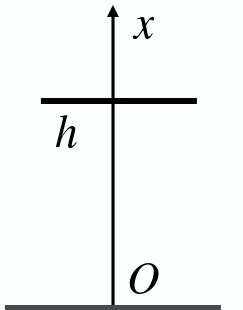
\includegraphics[scale=0.3]{img/vert.png}
\end{center}
Si hanno le seguenti condizioni iniziali:
\begin{itemize}
\item $t=t_0=0$
\item $x_0=h$
\item $\vec{v_0}=0$
\end{itemize}
Con queste premesse otteniamo:
\begin{itemize}
\item \textbf{Equazione del moto:}
$$\vec{x}(t)=x_0+\vec{v_0} t+\frac{1}{2} a  t^2$$
$$\downarrow$$
$$\vec{x}(t)=h-\frac{1}{2} g t^2$$
\item \textbf{Equazione della velocità:}
$$\vec{v}(t)=\vec{v_0}+a t$$
$$\downarrow$$
$$\vec{v}(t)=-g t$$
\end{itemize}
Posso quindi ottenere il tempo di caduta, ponendo $x=0$ nell'equazione del moto:
$$h-\frac{1}{2} g t^2=0\rightarrow t_c=\sqrt{\frac{2 h}{g}}$$
e posso ottenere la velocità al suolo:
$$v_c=v(t_c)=-g t_c=-g \sqrt{\frac{2 h}{g}}=-\sqrt{2 g h}$$
Imponiamo ora una velocità iniziale $-\vec{v_1}$, quindi verso il basso:
\begin{center}
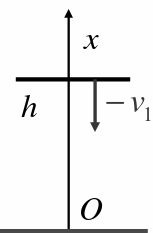
\includegraphics[scale=0.4]{img/vert2.png}
\end{center} 
Si hanno le seguenti condizioni iniziali:
\begin{itemize}
\item $t=t_0=0$
\item $x_0=h$
\item $\vec{v_0}=-\vec{v_1}$
\end{itemize}
\begin{itemize}
\item \textbf{Equazione del moto:}
$$\vec{x}(t)=x_0+\vec{v_0} t+\frac{1}{2} a  t^2$$
$$\downarrow$$
$$\vec{x}(t)=h-\vec{v_1}t-\frac{1}{2} g t^2$$
\item \textbf{Equazione della velocità:}
$$\vec{v}(t)=\vec{v_0}+a t$$
$$\downarrow$$
$$\vec{v}(t)=-\vec{v_1}-gt$$
\end{itemize}
Posso quindi ottenere il tempo di caduta, ponendo $x=0$ nell'equazione del moto:
$$h-\vec{v_1}t-\frac{1}{2} g t^2=0-\rightarrow \frac{1}{2} g t^2 +\vec{v_1}t-h=0$$
$$\downarrow$$
$$t_c=\frac{-\vec{v_1}\pm \sqrt{\vec{v_1}^2+2gh}}{g}$$
\begin{center}
\textit{ma $t<0$ non è una soluzione fisica, quindi tengo solo la soluzione col +}
\end{center}
$$t_c=-\frac{\vec{v_1}}{g}+\frac{1}{g}\sqrt{\vec{v_1}^2+2gh}$$
e posso ottenere la velocità al suolo:
$$v_c=-\vec{v_1}-gt_c=-\vec{v_1}-g\left[-\frac{\vec{v_1}}{g}+\frac{1}{g}\sqrt{\vec{v_1}^2+2gh}\right]=-\sqrt{\vec{v_1}^2+2gh}$$
Con una velocità iniziale verso il basso avremo un tempo di caduta inferiore e una velocità al suolo maggiore rispetto alla partenza da fermo.\\
Analizziamo ora il moto verticale di un punto materiale lanciato dal basso verso l'alto con velocità $\vec{v_2}$:
\begin{center}
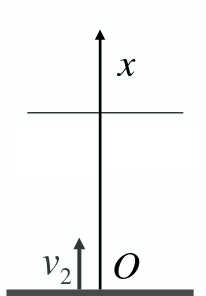
\includegraphics[scale=0.4]{img/vert3.png}
\end{center}
Si hanno le seguenti condizioni iniziali:
\begin{itemize}
\item $t=t_0=0$
\item $x_0=0$
\item $\vec{v_0}=\vec{v_2}$
\end{itemize}
\begin{itemize}
\item \textbf{Equazione del moto:}
$$\vec{x}(t)=x_0+\vec{v_0} t+\frac{1}{2} a  t^2$$
$$\downarrow$$
$$\vec{x}(t)=\vec{v_2}t-\frac{1}{2} g t^2$$
\item \textbf{Equazione della velocità:}
$$\vec{v}(t)=\vec{v_0}+a t$$
$$\downarrow$$
$$\vec{v}(t)=\vec{v_2}-gt$$
\end{itemize}
Inizialmente si ha $v>0$, finché il punto sale verso l'alto, fino a fermarsi. Con $v=0$ si ha l'altezza massima. Si ha quindi:
$$v=\vec{v_2}-gt=0\rightarrow t_{max}=\frac{\vec{v_2}}{g}$$
e quindi:
$$x_{max}=x(t_{max})=\vec{v_2}\frac{\vec{v_2}}{g}-\frac{1}{2}g\frac{\vec{v_2}^2}{g^2}=\frac{1}{2}\frac{\vec{v_2}^2}{g}$$
raddoppiando la velocità iniziale avrò quindi un'altezza 4 volte superiore. Da questp momento in poi di avrà la caduta libera da $h=x-max$ con $\vec{v_0}=0$:
$$t_c=\sqrt{\frac{2h}{g}}=\sqrt{\frac{2x_{max}}{g}}=\sqrt{\frac{2}{g}\left(\frac{1}{2}\frac{\vec{v_2}^2}{g}\right)}=\frac{\vec{v_2}}{g}$$
e quindi si avrà:
$$t_{tot}=t_{max}+t_c=\frac{2\vec{v_2}}{g}$$
\begin{comment}
\subsection{Moto Armonico}
Si ha la seguente equazione del moto per un \textit{moto armonico semplice} lungo un asse rettilineo:
$$\vec{x}(t)=Asin(\omega t+\varphi)$$
con:
\begin{itemize}
\item \textit{A} ampiezza, espressa in $m$ e costante
\item $\omega$ pulsazione, espressa in $s^{-1}$ e costante
\item $\varphi$ fase iniziale
\item $\omega t+\varphi$ è detta fase
\end{itemize}
Si ha inoltre:
\begin{itemize}
\item $sin(\omega t+\varphi)$ che è la traiettoria e si ha che $-1\geq sin(\omega t+\varphi)\leq 1$
\item $x_0=x(0)=asin\varphi$ è la posizione iniziale generica
\end{itemize}
$\vec{x}(t)=Asin(\omega t+\varphi)$ è una funzione periodica con periodo $T=2\pi$ (la posizione si ripete dopo ogni periodo \textit{T}). Consideriamo $T=t_2-t_1=2\pi$. Si ha quindi che:
$$x(t_2)=x(t_1)$$
$$\downarrow$$
$$Asin(\omega t_2+\varphi)=Asin(\omega t_1+\varphi)$$
$$\downarrow$$
$$(\omega t_2+\varphi)-(\omega t_1+\varphi)=2\pi$$
$$\downarrow$$
$$\omega(t_2-t_1)=2\pi$$
$$\downarrow$$
$$T=\frac{2\pi}{\omega}$$
Si ha quindi che:
\begin{itemize}
\item $\omega=\frac{2\pi}{T}$, la pulsazione è inversamente proporzionale al periodo
\item \textbf{Frequenza:} $\nu =\frac{1}{T}$ quindi $\omega=2\pi\ni$
\end{itemize}
Pulsazione e frequenza sono indipendenti dall'ampiezza.\\
Posso ora trovare velocità ed accelerazione dall'equazione del \\moto $\vec{x}(t)=Asin(\omega t+\varphi)$:
\begin{itemize}
\item \textbf{velocità:} $\vec{v}(t)=\frac{d\vec{x}(t)}{dt}=A\omega\, cos(\omega t+\varphi)$
\item \textbf{accelerazione:} $\vec{v}(t)=\frac{d\vec{v}(t)}{dt}=\frac{d^2\vec{x}(t)}{dt^2}=-A\omega^2 \,sin(\omega t+\varphi)=-\omega^2 \vec{x}(t)$
\end{itemize}
Ampiezza di $\vec{v}(t)$ e \textit{a(t)} dipendono dalla pulsazione. Le tre curve \textit{$\vec{x}(t)$}, $\vec{v}(t)$ e \textit{a(t)} hanno lo stesso andamento ma sono sfasate tra loro. Ricordando che $sin(\alpha+\frac{\pi}{2}=cos \alpha$ e che $sin(\alpha+\pi)=-sin\alpha$ notiamo che $\vec{v}(t)$ è sfasata di $\frac{\pi}{2}$ rispetto a \textit{$\vec{x}(t)$} (\textit{quadratura di fase}) e che \textit{a(t)} è sfasata di $\pi$ rispetto a \textit{$\vec{x}(t)$} (\textit{opposizione di fase}) 
\begin{center}
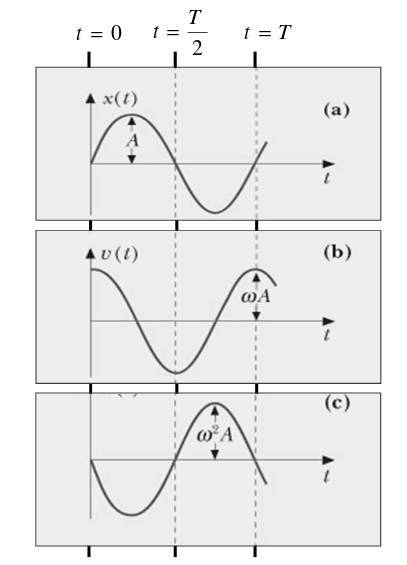
\includegraphics[scale=0.5]{img/arm.png}
\end{center}
\end{comment}
\subsection{Moto nel Piano}
Si passa ora al moto in 2 dimensioni quindi con una traiettoria curva (e non più una retta).\\
Si introducono le coordinate cartesiane (${x}(t)$ e $y(t)$) e quelle polari ($r(t)$ e $\vartheta(t)$). Si hanno le seguenti formule per il passaggio da coordinate cartesiane a polari:
$$r=\sqrt{x^2+y^2}$$
$$tan\,\vartheta=\frac{y}{x}$$
e le seguenti per il passaggio da coordinate polari a cartesiane:
$$x=r\,cos\,\vartheta$$
$$y=r\,sin\,\vartheta$$
\begin{center}
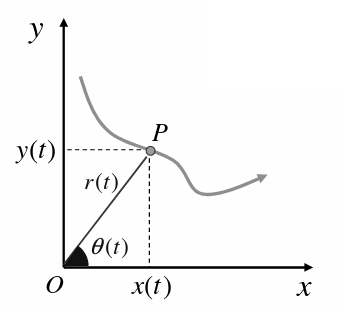
\includegraphics[scale=0.4]{img/pia.png}
\end{center}
Il moto di $P$ è descritto attraverso l'evoluzione del vettore posizione:
$$\vec{r}(t)\equiv (\vec{x}(t),y(t))$$
Si introducono inoltre i versori degli assi $\vec{u}_x,\,\vec{u}_y$, ricordando che $|\vec{u}_x|=|\vec{u}_y|=1$ e che i versori restano fissi nel tempo. Si ottiene quindi:
$$\vec{r}(t)=\vec{x}(t)\vec{u}_x+y(t)\vec{u}_y$$
\begin{center}
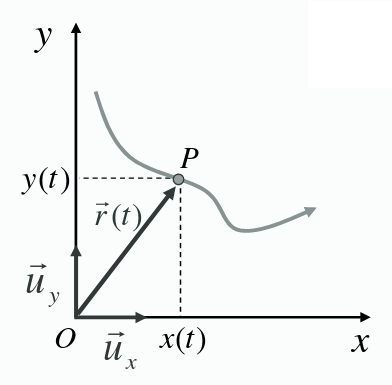
\includegraphics[scale=0.4]{img/pia2.png}
\end{center}
Suppongo ora la traiettoria fissata e nota a priori. Fissata un'origine $O$, una posizione $s(t)$ e la velocità $v=\frac{ds}{dt}$ si ha che il moto è completamente determinato. Si ha una generalizzazione del moto rettilineo su una traiettoria curva.\\
Prendiamo ora in considerazione il seguente caso:
\begin{center}
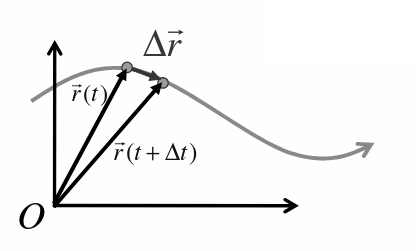
\includegraphics[scale=0.4]{img/pia3.png}
\end{center}
si ha il vettore spostamento:
$$\Delta\vec{r}(t)=\vec{r}(t+\Delta t)-\vec{r}(t)$$
e il vettore velocità media:
$$\vec{v}_m\equiv\frac{\Delta\vec{r}}{\Delta t}$$
e il vettore velocità istantanea:
$$\vec{v}(t)=\lim_{\Delta t\to 0}\frac{\Delta\vec{r}}{\Delta t}=\lim_{\Delta t\to 0}\frac{\vec{r}(t+\Delta t)-\vec{r}(t)}{\Delta t}=\frac{d\vec{r}}{dt}$$
al limite $\Delta t\to 0$ lo spostamento infinitesimo si dispone sulla tangente alla traiettoria nel punto $P$: 
$$d\vec{r}=ds\vec{u}_T$$
con $|\vec{u}_T|=1$ versore della tangente che indica una direzione variabile nel tempo. Per il vettore velocità avremo:
$$\vec{v}=\frac{d\vec{r}}{dt}=\frac{ds}{dt}\vec{u}_T=v\vec{u}_T$$
con $v$ indicate il modulo della velocità e $\vec{u}_T$ la direzione.
\newpage
 Quanto appena descritto è visualizzabile nelle seguenti immagini:
\begin{center}
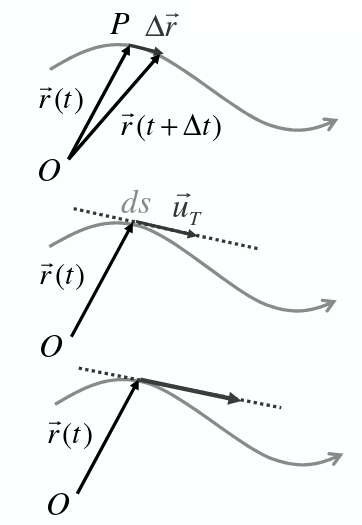
\includegraphics[scale=0.4]{img/pia4.png}
\end{center}
Analizziamo ora meglio la velocità nelle componenti cartesiane. Essendo $\vec{v}_m=\frac{\Delta\vec{r}}{\Delta t}$ e $\vec{r}(t)=\vec{u}_x+y(t)\vec{u}_y$ si ottiene:
$$\vec{v}=\frac{dx}{dt}\vec{u}_x+\frac{dy}{dt}\vec{u}_y=v_x\vec{u}_x+v_y\vec{u}_y$$
con il modulo della velocità:
$$v=|\vec{v}|=\sqrt{v_x^2+v_y^2}$$
Ecco un'immagine di quanto detto:
\begin{center}
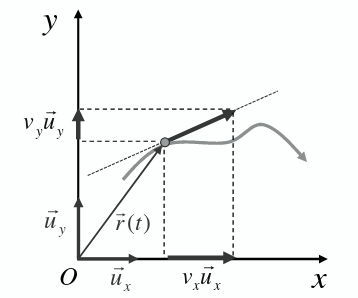
\includegraphics[scale=0.6]{img/pia5.png}
\end{center}
Passiamo alle componenti polari. Essendo $\vec{v}_m=\frac{\Delta\vec{r}}{\Delta t}$ e $\vec{r}(t)=r(t)\vec{u}_r(t)$ (col versore $\vec{u}_r$ mostrato in figura) si ottiene:
$$\vec{v}=\frac{d}{dt}(r\vec{u}_r)=\frac{dr}{dt}\vec{u}_r+r\frac{d\vec{u}_r}{dt}=\frac{dr}{dt} \vec{u}_r+r\frac{d\vartheta}{dr}\vec{u}_\vartheta$$
in quanto solitamente la derivata di un versore è: 
$$\frac{d\vec{u}}{dt}=\frac{\vec{u}(t+dt)-\vec{u}(t)}{dt}=\frac{d\vartheta}{dt}\vec{u}_\bot$$
Ecco un'immagine di quanto detto:
\begin{center}
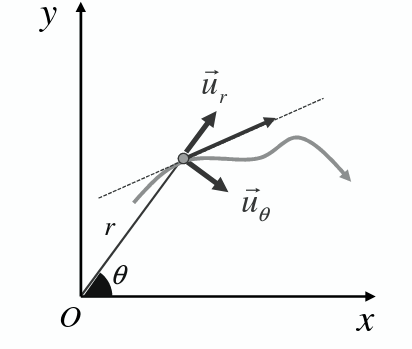
\includegraphics[scale=0.5]{img/pia6.png}
\end{center}
Possiamo approfondire ancora lo studio della velocità in componenti polari infatti:
$$\vec{v}=\underbrace{\frac{dr}{dt} \vec{u}_r}_{\vec{v_r}}+\underbrace{r\frac{d\vartheta}{dr}\vec{u}_\vartheta}_{\vec{v}_\vartheta}$$
con:
\begin{itemize}
\item $\vec{v_r}$ è la \textbf{velocità radiale} e $|\vec{v_r}|=\frac{dr}{dt}$  è la variazione di $r$
\item $\vec{v_\vartheta}$ è la \textbf{velocità traversa} e $|\vec{v_\vartheta}|=r\frac{d\vartheta}{dt}$ è la variazione della direzione
\end{itemize}
quindi:
$$\vec{v}=\vec{v_r}+\vec{v_\vartheta}$$
e quindi:
$$|\vec{v}|=\sqrt{v_r^2+v_\vartheta^2}=\sqrt{\left(\frac{dr}{dt}\right)^2+r^2\left(\frac{d\vartheta}{dt}\right)^2}$$
\newpage
Ecco un'immagine che spiega quanto detto:
\begin{center}
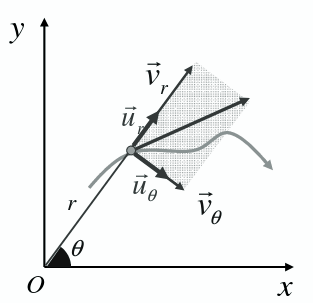
\includegraphics[scale=0.5]{img/pia7.png}
\end{center}
Passiamo ora all'accelerazione nel piano. Essa è, come sappiamo, la variazione della velocità $\vec{v}=v\vec{u}_T$ ma, se nel moto rettilineo è solo la variazione del modulo, nel moto del piano si ha anche la variazione della direzione. Iniziamo sapendo che $\vec{a}=\frac{d\vec{v}}{dt}$. Quindi:
$$\vec{a}=\frac{d}{dt}(v\vec{u}_t)=\frac{dv}{dt}\vec{u}_T+v\frac{d\vec{u}_t}{dt}$$
ricordando la derivata di un versore si ottiene:
$$\vec{a}=\frac{dv}{dt}\vec{u}_T+v\frac{d\phi}{dt}\vec{u}_N$$
con:
\begin{itemize}
\item $\vec{u}_N$ versore perpendicolare al versore tangente
\item $\frac{dv}{dt}\vec{u}_T$ variazione del modulo velocità, detta $\vec{a}_T$ \textbf{accelerazione tangenziale}
\item $v\frac{d\phi}{dt}\vec{u}_N$ variazione della direzione, detta $\vec{a}_T$ \textbf{accelerazione normale o centripeta}
\end{itemize}
quindi:
$$\vec{a}=\vec{a}_T+\vec{a}_N$$
procedendo con l'analisi della traiettoria si nota come essa possa essere approssimata da una circonferenza con un certo raggio $R$ che può essere usato come raggio di curvatura. Si ha quindi $ds=R\,d\phi$ e quindi:
$$\frac{d\,\phi}{dt}=\frac{1}{R}\frac{ds}{dt}=\frac{1}{R}v$$
Posso quindi sostituire $\frac{d\,\phi}{dt}$ nella formula precedentemente trovata dell'accelerazione ottenendo:
$$\vec{a}=\frac{dv}{dt}\vec{u}_T+\frac{v^2}{R}\vec{u}_N$$
quindi $\vec{a}_N$ può anche essere indicata con $\vec{a}_N=\frac{v^2}{R}\vec{u}_N$. Da questi ultimi due risultati si intuiscono due cose:
\begin{enumerate}
\item se $r\to\infty$ si ha $\vec{a}_N=0$ e quindi un moto rettilineo
\item se $\frac{dv}{dt}=0$ si ha $\vec{a}_T=0$ e quindi un moto curvilineo uniforme con solo il cambiamento della direzione
\end{enumerate}
Si ha infine il modulo dell'accelerazione:
$$a=|\vec{a}|=\sqrt{\left(\frac{dv}{dt}\right)^2+\frac{v^4}{R^2}}$$
Ecco un'immagine di quanto detto:
\begin{center}
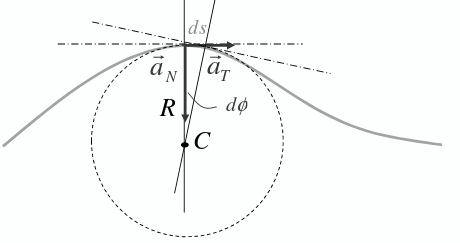
\includegraphics[scale=0.5]{img/pia8.png}
\end{center}
Proiettiamo ora l'accelerazione sugli assi del sistema cartesiano:
$$\vec{a}=\frac{dv_x}{dt}\vec{u}_x+\frac{dv_y}{dt}\vec{u}_y=a_x\vec{u}_x+a_y\vec{u}_y$$
analizziamo anche quanto succede sul piano:
\begin{center}
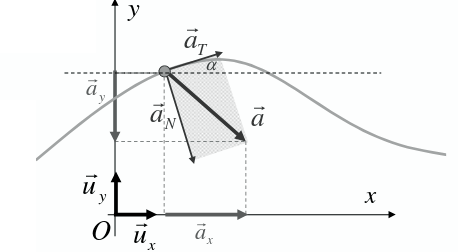
\includegraphics[scale=0.6]{img/pia9.png}
\end{center}
Possiamo ora scrivere le componenti cartesiane in funzione di quella tangenziale e di quella centripeta:
\begin{itemize}
\item per l'ascisse:
$$a_x=(a_T)_x+(a_N)_x=a_tcos\,\alpha+a_ncos\left(\frac{\pi}{2}-\alpha\right)=\frac{dv}{dt}cos\,\alpha+\frac{v^2}{R}sin\,\alpha$$
\item per l'ordinata:
$$a_y=\frac{dv}{dt}sin\,\alpha-\frac{v^2}{R}cos\,\alpha$$
\end{itemize}
\subsection{Moto Circolare}
Si tratta di un caso particolare di moto curvilineo nel piano. In generale si ha il modulo della velocità non uniforme. Si hanno quindi:
\begin{itemize}
\item \textit{coordinate polari}:
\begin{itemize}
\item angolo $\theta(t)$
\item raggio $r(t)=R=costante$
\end{itemize}
\item \textit{coordinate curvilinee}:
\begin{itemize}
\item posizione misurata lungo la traiettoria $s(t)=R\theta (t)$
\end{itemize}
\item \textit{coordinate cartesiane:}
\begin{itemize}
\item $\vec{x}(t)=R\,cos\,\theta(t)$
\item $y(t)=R\,sin\,\theta(t)$
\end{itemize}
\end{itemize}
ovvero:
\begin{center}
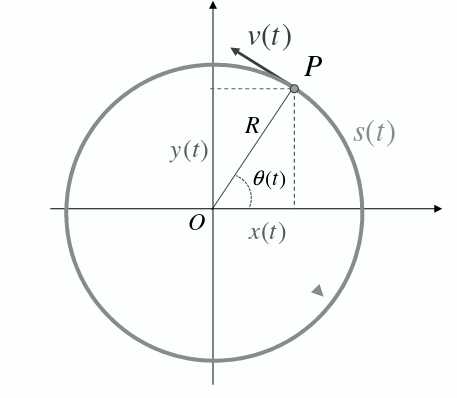
\includegraphics[scale=0.52]{img/cir.png}
\end{center}
Iniziamo ad analizzare il moto circolare. Considero il punto $P$ in due istanti $t$ e $t+\Delta t$. Quindi avrò $\theta (t)=\theta_1$ e $\theta(t+\Delta t)=\theta_2$. Nel complesso si ha $\Delta \theta= \theta_2-\theta_1$:
\begin{center}
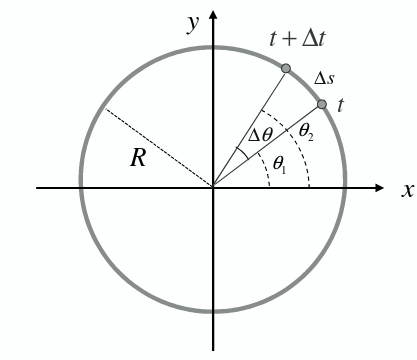
\includegraphics[scale=0.52]{img/cir2.png}
\end{center}
Si definisce innanzitutto la velocità angolare media:
$$\omega_m=\frac{\Delta\theta}{dt}$$
mentre per la velocità angolare istantanea si ha:
$$\omega=\lim_{\Delta t\to 0}\frac{\Delta\theta}{dt}=\frac{d\theta}{dt}$$
Si indica ora la velocità angolare in funzione di $v$ e $R$, ricordando che $ds=Rd\theta$:
$$\omega=\frac{d\theta}{dt}=\frac{1}{R}\frac{ds}{dt}=\frac{v}{R}$$
quindi la velocità angolare è proporzionale al modulo della velocità ed inversamente proporzionale al raggio. Inoltre $v=\omega R$. Partiamo da qui per approfondire la velocità nel moto circolare. Sappiamo che in generale nel moto curvilineo si ha: $\vec{v}=\frac{dr}{dt}\vec{u_r}+r\frac{d\theta}{dt}\vec{u_\theta}$. Si ha che $\frac{dr}{dt}=0$ quindi:
$$\vec{v}=R\frac{d\theta}{dr}\vec{u}_\theta=R\omega\vec{u}_\theta$$
\newpage
in quanto $R$ è costante e quindi si ha come modulo della velocità:
$$\vec{v}(t)=|\vec{v}(t)|=\omega(t)R$$
graficamente si ha:
\begin{center}
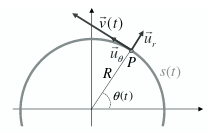
\includegraphics[scale=0.9]{img/cir3.png}
\end{center}
Si ha inoltre che se si parla di moto circolare uniforme si ha che $v=\omega R$ è costante in quanto $\omega$ è costante.\\
Passiamo all'accelerazione nel moto circolare uniforme. Si ha solo l'accelerazione centripeta in quanto $\frac{dv}{dt}=0$
$$\vec{a}=\frac{v^2}{R}\vec{U}_N$$
con $v^2$ costante e si ha il modulo dell'accelerazione pari a:
$$a=|\vec{a}|=\frac{v^2}{R}=\frac{(\omega R)^2}{R}=\omega^2 R=\omega \, v$$
Quindi per il moto lungo la traiettoria si ha:
\begin{itemize}
\item $s(t)=s_0+vt$
\item $\theta(t)=\theta_0+\omega t$
\end{itemize}
e nel moto circolare uniforme si può notare un moto periodico con periodo:
$$T=\frac{2\pi R}{v}=\frac{2\pi R}{\omega R}=\frac{2\pi}{\omega}$$
vediamo ora l'accelerazione in caso di moto non uniforme, quindi con $\vec{a}=\vec{a}_T+\vec{a}_N$ e con $\vec{v}(t)=\omega(t)R$. Definisco un'accelerazione angolare media:
$$\alpha_m=\frac{\omega_2-\omega_1}{\Delta t}=\frac{\Delta\omega}{\Delta t}$$
e l'accelerazione angolare istantanea, si ricorda che $\omega=\frac{v}{r}$:
$$\alpha=\lim_{\Delta t\to 0}\frac{\Delta\omega}{\Delta t}=\frac{d\omega}{dt}=\frac{1}{R}\frac{dv}{dt}=\frac{1}{R}a_T$$
\newpage
visivamente:
\begin{center}
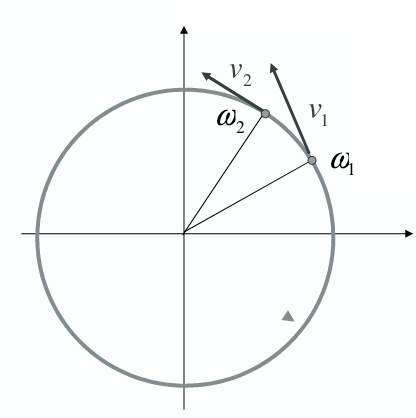
\includegraphics[scale=0.4]{img/cir4.png}
\end{center}
Possiamo quindi riscrivere accelerazione normale e tangenziale in funzione di quantità angolari:
\begin{itemize}
\item $a_N=\frac{v^2}{R}\xrightarrow{v=\omega R} a_N=\omega^2 R$
\item $a_T=\frac{dv}{dt}\xrightarrow{v=\omega R} a_T=\frac{d\omega}{dt}R=\alpha R$
\end{itemize}
quindi:
$$\vec{a}=\alpha R\vec{u}_T+\omega^2 R\vec{u}_N= R(\alpha \vec{u}_T+\omega^2 \vec{u}_N)$$
quindi infine:
\begin{itemize}
\item $\omega(t)=\omega_0+\int_{t_0}^t \alpha dt=\omega_0+\alpha \int_{t_0}^t dt=\omega_0+\alpha t$ in quanto $t_0=0$
\item $\theta(t)=\theta_0+\int_{t_0}^t \omega (t)dt=\theta_0+\int_{t_0}^t (\omega_0+\alpha t)dt=\theta_0+\omega_0t+\frac{1}{2}\alpha t^2$, dove si nota l'analogia con l'accelerazione nel moto rettilineo
\item $a_N=\omega^2 R=(\omega_0+\alpha t)^2 R$
\end{itemize}
Diamo nuovamente un'occhiata alla velocità angolare $\omega=\frac{d\theta}{dt}=\frac{v}{R}$. Si ha che è una quantità scalare. Studiamo ora la notazione vettoriale di $\vec{\omega}$. Questo vettore ha direzione ortogonale alla circonferenza e , visto dalla punta di $\vec{\omega}$ il moto appare antiorario. SI ha quindi che $\vec{\omega}\times \vec{r}=\vec{v}$ e:
$$|\vec{v}|=\omega Rsin\,\frac{\pi}{2}=\omega R$$
anche se il vettore $\vec{\omega}$si può applicare a qualunque punto dell'asse $z$, ottenendo:
$$|\vec{v}|=\omega Rsin\,\phi=\omega R$$
\newpage
graficamente si ha a sinistra il caso con applicazione sull'origine normale e a destra il caso applicazione in un punto a scelta:
\begin{center}
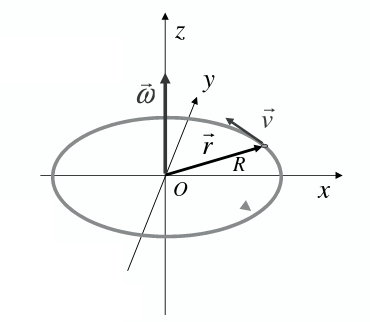
\includegraphics[scale=0.5]{img/cir5.png}
\quad
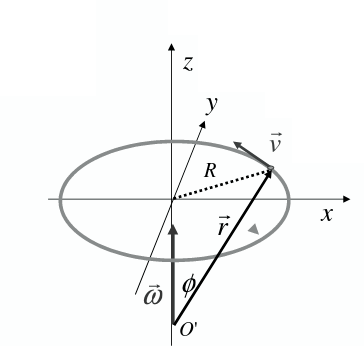
\includegraphics[scale=0.5]{img/cir6.png}
\end{center}
\subsection{Moto Parabolico}
Consideriamo il moto di un punto materiale lanciato da terra (con angolo $\theta_0$) con una certa velocità iniziale $v_0$:
\begin{center}
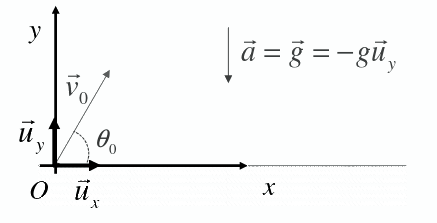
\includegraphics[scale=0.5]{img/par.png}
\end{center}
posto $t_0=0$ e $\vec{r}(t_0)=0$
otteniamo per la velocità:
$$\vec{v}(t)=\vec{v}(t_0)+\int_{t_0}^t\vec{a}(t)\,dt=\vec{v_0}-g\vec{u}_y\int_{t_0}^t dt=\vec{v}_0-gt\vec{u}_y$$
$$\downarrow$$
$$
\begin{cases}
v_x=v_0cos\theta_0\\
v_y=v_0sin\theta_0-gt
\end{cases}
$$
\newpage
e per la posizione:
$$\vec{r}(t)=\vec{r}(t_0)+\int_{t_0}^t\vec{v}(t)\,dt$$
$$\downarrow$$
$$
\begin{cases}
x=x(t)=\int_{t_0}^t v_x=(v_0cos\theta_0)t\\
y=y(t)=\int_{t_0}^t v_y=(v_0sin\theta_0)t-\frac{1}{2}gt^2
\end{cases}
$$
notiamo che la componente $x$ rappresenta un moto rettilineo uniforme mentre quella $y$ un moto uniformemente accelerato. Passiamo ora al calcolo della traiettoria $y(x)$. Dall'equazione di $x(t)$ otteniamo:
$$t=\frac{x}{v_0cos\theta_0}$$
quindi:
$$y(x)=(v_0sin\theta_0)\frac{x}{v_0cos\theta_0}-\frac{1}{2}g\frac{x^2}{v_0^2cos\theta^2_0}$$
$$\downarrow$$
$$y(x)=(tan\theta_0)x-\frac{g}{2v_0^2cos^2\theta_0}x^2$$
ovvero l'equazione di una parabola con asse verticale, infatti:
\begin{center}
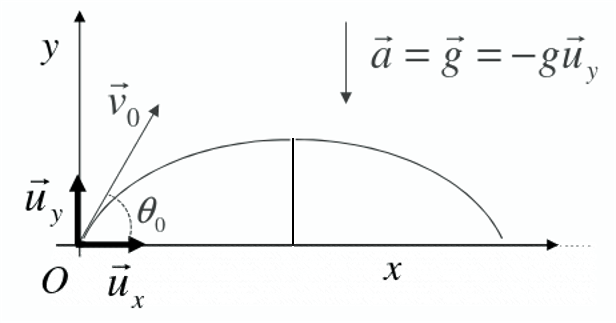
\includegraphics[scale=0.5]{img/par2.png}
\end{center}
\newpage
Studiamo ora la gittata, che si ha con $y(x)=0$:
\begin{center}
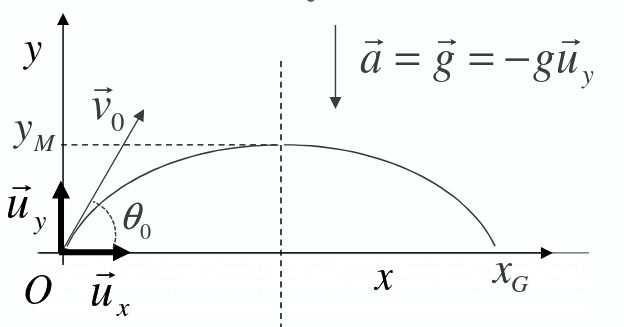
\includegraphics[scale=0.4]{img/par3.png}
\end{center}
Quindi, essendo $y(x)=0$, si ha:
$$tan\theta_0=\frac{g}{2v_0^2cos^2\theta_0}$$
quindi:
$$x_G=\frac{2v_0^2}{g}cos^2\theta_0 tan\theta_0=\frac{2v_0^2}{g}cos\theta_0 sin\theta_0$$
$$\downarrow$$
$$x_G=\frac{v_0^2}{g}sin(2\theta_0)$$
e, fissata la velocità iniziale si ha la gittata massima con $sin(2\theta_0)=1$ (quindi con $\theta_0=\frac{\pi}{4}=45^{\circ}$). Si ha quindi:
$$x_{G_{max}}=\frac{v_0^2}{g}$$
la parabola è simmetrica rispetto all'asse e a $x_M$ si ha l'altezza massima $y_M=y(x_M)$. Si ha:
$$x_M=\frac{1}{2}\frac{v_0^2}{g}sin(2\theta_0)$$
e, mettendo $x_M$ nella formula della traiettoria, si ottiene:
$$y_M=\frac{v_0^2}{2g}sin^2\theta_0$$
che è l'altezza massima lungo la traiettoria.
Ne segue che l'altezza massima si ha sulla verticale (con $\theta_0=\frac{\pi}{2}$) e quindi si ha l'altezza massima pari a:
$$Y_{M_{max}}=\frac{v_0^2}{2g}$$
Possiamo ora calcolare il tempo di volo, ovvero il tempo impiegato a raggiungere la gittata $x_G$:
$$t_G=\frac{x_G}{v_x}=\frac{v_0^2}{g}sin(2\theta_0)\frac{1}{v_0cos\theta_0}$$
$$\downarrow$$
$$t_G=\frac{2v_0}{g}sin\theta_0$$
che con $sin\theta_0=1$, ovvero con $\theta_0=\frac{\pi}{2}$ (sulla verticale), raggiunge il suo massimo:
$$t_{G_{max}}=\frac{2v_0}{g}$$
si hanno inoltre le seguenti velocità finali:
$$\begin{cases}
v_x(t_G)=v_x(t_0)=v_0cos\theta_0\\
v_y(t_G)=-v_y(t_0)=-v_0sin\theta_0
\end{cases}$$
Vediamo ora un punto materiale lanciato orizzontalmente da altezza $h$.
\begin{center}
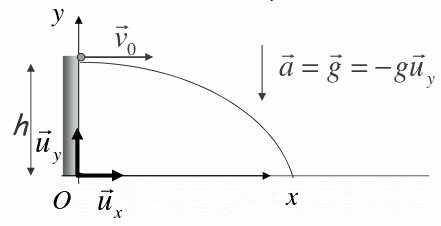
\includegraphics[scale=0.6]{img/ori.png}
\end{center}
è un moto parabolico con condizioni iniziali diverse:
\begin{itemize}
\item $x(0)=0$
\item $y(0)=h$
\item $v_x(0)=v_0$
\item $v_y(0)=0$
\end{itemize}
con la seguente equazione  del moto:
$$\begin{cases}
x(t)=v_0t\\
y(t)=h-\frac{1}{2}gt^2
\end{cases}$$
che implicano:
$$\begin{cases}
v_x(t)=v_0\\
v_y(t)=-gt
\end{cases}$$
si hanno quindi:
\begin{itemize}
\item tempo di volo: $t=\frac{x}{v_0}$
\item traiettoria: $y(x)=h-\frac{g}{2v_0^2}x^2$
\item tempo di caduta: $y(t)=0\to h-\frac{1}{2}gt^2=0\to t_c=\sqrt{\frac{2h}{g}}$
\item gittata: $x(t_c)=x_G=v_0t_c=v_0\sqrt{\frac{2h}{g}}$
\item velocità finale: $v_x(t_c)=v_0$ \textit{e} $v_y(t_c)=-\sqrt{2gh}\to v_c=\sqrt{v_0^2+2gh}$
\end{itemize}
\subsection{Esercizi}
prodotto scalare:
$$\vec{a} \cdot \vec{b}=ab\,cos\theta$$
prodotto vettoriale:
$$\vec{a} \times \vec{b}=\vec{c}\to |\vec{c}|=ab\,sin\theta$$
\begin{esercizio}
si ha una strada rettilinea di 5.2km percorsa in auto a 43km/h, dopo si ha un altro percorso di 1.2km (fatto in 27m). Trovo velocità media nei due tratti:\\
%aggiungo grafico
$$v_{med}=\frac{\Delta x}{\Delta t}$$
$$\Delta x = \Delta x_1+\Delta x_2= 5.2+1.2=6.4km$$
$$\Delta t = \Delta t_1+\Delta t_2= \frac{\Delta x_1}{v}+\Delta t_2=\frac{5.2}{43}+0.45=0.12+0.45=0.57h$$
$$v_{med}=\frac{\Delta x}{\Delta t}=\frac{6.4}{0.57}=11km/h$$
ora torna alla macchina, tornando indietro di 1.2km in 35m, quindi la nuova velocità media totale sarà:
$$v_{med2}=\frac{5.2}{0.57+0.58}=4.5km/h$$
\textit{sistemare parte finale}
\end{esercizio}
\begin{esercizio}
negli anni '60 c'è stato il record di velocità al suolo con 631km/h in 3.72s. L'accelerazione media è maggiore di quella di gravità?
$$a_{med}=\frac{\Delta v}{\Delta t}=\frac{631}{3.6}\frac{1}{3.72}=47,2m/s^2$$
che è maggiore di 9.81
\end{esercizio}
\begin{esercizio}
la metro va da A a B. Quando parte accelera con 1.2m$/s^2$, per metà tratta accelera così positivamente e poi frena con lo stesso modulo. Tra A e B ci sino 1100m. Calcolo tempo e velocità massima:
$$v_{max}=v\frac{\Delta x}{2}=\sqrt{2a\Delta x\frac{1}{2}}=\sqrt{a\Delta x}=\sqrt{1.2*1100}=36,3m/s$$
$$v=v_0+at\to t=\frac{v_{fin}}{a}=\frac{36.3}{1.2}=30.3s$$
$$\Delta t_{tot}=30.3\cdot 2= 60.6s$$
in quanto accelera e frena con lo stesso modulo
\end{esercizio}
\begin{esercizio}
un tizio urla in un pozzo e l'eco gli torna dopo 2s. Quanto è profondo il pozzo ($v_{suono}=344m/s$)
$$2\Delta x= v\Delta t\to t=\frac{344\cdot 2}{2}=344m$$
\end{esercizio}
\begin{esercizio}
Un aereo per staccarsi dalla pista deve avere una velocità finale di 360km/h. La pista è lunga 1,8km. Si ha accelerazione costante. Qual è l'accelerazione minima?
$$v_{fin}^2=v_0^2+2a\Delta x\to a=\frac{360}{3.6}\frac{1}{2\cdot 1.8\times 10^3}=2.7m/s^2$$
\end{esercizio}
\begin{esercizio}
Un tizio fa cadere una chiave inglese da un grattacielo. Dov'è la chiave dopo 1.5s?
$$\Delta x= -\frac{1}{2}gt^2=-\frac{9.81\cdot 1.2^2}{2}=-11m$$
negativo nel mio sistema di riferimento 
\end{esercizio}
\begin{esercizio}
lancio una palla in alto con $v_0=12m/s$, quanto ci impiega ad arrivare alla massima altezza?
$$v_f=v_0-gt\to t=\frac{v_0}{g}=\frac{12}{9.81}=1.2s$$
quanta strada fa?
$$x=-\frac{v_0^2}{2g}=-\frac{12^2}{2\cdot (-9.81)}=7,3m$$

quanto impiega la palla per arrivare a 5m sopra il punto di lancio?
$$x=v_0t-\frac{1}{2}gt^2\to \frac{1}{2}9,81t^2+12t+5=0$$
$$\downarrow$$
$$t=\frac{12\pm \sqrt{12^2-4\frac{9,81}{2}5}}{2,45}=\begin{cases}
0,53s\\
1,9s
\end{cases}$$
sappiamo che per arrivare all'altezza massima impiega 1,2s, quindi impiegherà 0,53s per arrivare a 5m e 1,9s per salire all'apice e scendere nuovamente a 5m
\end{esercizio}
\begin{esercizio}
Un aereo getta aiuti umanitari ad una quota di 1200m volando a 430km/h. Calcolo a quale angolo devono essere gettati gli aiuti?
$$
\begin{cases}
x=v_{0_x}t\\
y=v_{0_y}t-\frac{1}{2}gt^2=-\frac{1}{2}gt^2
\end{cases}
$$ 
$$t=\sqrt{\frac{2y}{g}}=\sqrt{\frac{2400}{9,81}}=15,6s$$
$$\downarrow$$
$$x=\frac{430}{3,6}\cdot 15,6=1863m$$
$$\downarrow$$
$$tan(\frac{\pi}{2}-\theta)=\frac{\Delta x}{\Delta y}=\frac{1869}{1200}$$
$$\downarrow$$
$$\frac{\pi}{2}-\theta=arctan\left(\frac{1869}{1200}\right)=57^{\circ}$$
\end{esercizio}
\begin{esercizio}
\textit{una pallina viene scagliata contro un muro a 25m/s. Dopo l'impatto torna indietro a -22m/s. Calcolo l'accelerazione media sapendo che l'impatto dura 3,5ms}
$$a_{med}=\frac{\Delta v}{\Delta t}=\frac{25-(-22)}{3,5\times 10^{-3}}=\frac{47}{3,5\times 10^{-3}}$$
\end{esercizio}
\begin{esercizio}
\textit{una pallina viene lanciata su uno scalino. Sapendo che viene lanciata con un angolo di 60 gradi a 42m/s e che atterra dopo 5,53s calcolo l'altezza del gradino}
$$y(5,53)=v_{0_y}t-\frac{1}{2}gt^2=42sin\left(\frac{\pi}{3}\right()-\frac{1}{2}\cdot 9,8\cdot 5,53^2=51,8m$$
calcolo la velocità d'impatto:\\
calcolo prima la velocità sulle ordinate:
$$v_y(5,53)=v_{0_y}-gt=v_0sin\left(\frac{pi}{3}\right)-9,81\cdot 5,53=-17m/ s$$
e infine:
$$v=\sqrt{v_{o_y}^2
v_{0_x}^2}=\sqrt{21^2+(-17)^2}=27m/ s$$
\end{esercizio}
\begin{esercizio}
\textit{ho una pallina che si muove lungo un cerchio di raggio 0,1m. Si ha la velocità iniziale pari a 0,05m/s e dopo 1s si trova a 0,08m. Calcolo accelerazione tangenziale e centripeta a 1s}:\\
parto dall'accelerazione tangenziale
$$x(t)=v_0t+\frac{1}{2}a_Tt^2$$
$$\downarrow$$
$$8\times 10^{-2}=0,05\times 1\frac{1}{2}a_T(1)^2$$
$$\downarrow$$
$$a_T=6\times 10^{-2}m/s^2$$
passo all'accelerazione centripeta:
$$a_N(1)=\frac{v(1)^2}{R}=\frac{(v_0+a_Tt^2)^2}{R}=0,121m/s^2$$
????????????????????
\end{esercizio}
\begin{esercizio}
\textit{Un oggetto posto a 1,2m di altezza viene spinto in avanti, cadendo a 1,5m di distanza. Calcolo il tempo di volo}\\
mi basta il tempo su y:
$$\Delta y= v_{0_y}t+\frac{1}{2}gt^2$$
$$\downarrow v_{0_y}=0$$
$$t=\sqrt{\frac{2\Delta y}{g}}=\sqrt{\frac{2\cdot 1,2}{9,81}}=0,49s$$
trovo ora la velocità su x:
$$v_{0_x}=\frac{\Delta x}{\Delta t}=\frac{1,5}{0,49}=3m/s$$
\end{esercizio}
\newpage
\section{Dinamica}
La dinamica studia le cause del moto. Si studia un punto materiale con una certa massa, detta anche \textit{massa inerziale}, (che è una proprietà intrinseca dei corpi, è una quantità scalare, mentre il peso è una quantità scalare rivolta verso il basso e dipendente dall'accelerazione di gravità, e si esprime in \textit{kg} secondo il \textit{SI}) in un certo ambiente che condiziona quel punto materiale. Si hanno le tre leggi di Newton:
\begin{itemize}
\item \textbf{Prima legge:} \textit{in assenza di forze esterne (ovvero la somma delle forze vettoriali applicate è 0) su un corpo si ha che lo stesso non cambia velocità (il suo moto non cambia)}; si ha quindi un \textbf{sistema inerziale}. Nel caso di presenza di forze nel sistema di ha un \textbf{sistema non inerziale}, dove agiscono forze \textbf{non apparenti}
\item \textbf{Seconda legge:} \textit{si ha una relazione tra forza (espressa in Newton, N, è una quantità vettoriale) e accelerazione. Si ha inoltre la presenza della massa in questa relazione. Si scopre sperimentalmente che vale la seguente relazione, in quanto massa e accelerazioni sono inversamente proporzionali:}
$$\vec{F}=m\vec{a}\to \vec{a}=\frac{\vec{F}}{m}$$
$$\downarrow$$
$$\frac{d^2\vec{x}(t)}{dt^2}=\frac{\vec{F}(t)}{m}$$
ovviamente posso anche scomporre:
$$\vec{F}\equiv
\begin{cases}
\vec{F}_z=m\vec{a}_x\\
\vec{F}_z=m\vec{a}_y\\
\vec{F}_z=m\vec{a}_z\\
\end{cases}$$
\item \textbf{Terza legge:} \textit{è il \textbf{principio di azione-reazione}}
\end{itemize}
%aggungi immagine vettori forze
%approfindisci forze apparenti
Un Newton è: 
$$N=kg\frac{m}{s^2}$$
\newpage
\subsection{Forza elastica}
Si definisce la legge di Hooke:
$$\vec{F}=-k\Delta \vec{x}$$
dove $k$ è la costante elastica. La forza elastica si oppone all'allungamento della molla. Quindi si ha:
$$\vec{F}(x)=-k(x-x_0)=m\vec{a}$$
$$\downarrow$$
$$\vec{a}=\frac{-k(x-x_0)}{m}$$
Il moto poi dell'estremità della molla viene espresso da un moto armonico.
\subsection{Lavoro e Energia}
\subsubsection{Lavoro}
La \textit{conservazione dell'energia} è un principio base della fisica. Ci sono delle combinazioni matematiche di cinematica e forze che costruiscono l'energia, che non è frutto di un'indagine sperimentale. L'energia va individuata i vari aspetti del sistema considerato. Un sistema può essere formato da più punti materiali e l'energia può studiare i sistemi senza doverne scomporre le parti. Se un sistema non scambia energia con l'esterno mantiene costante l'energia interna.\\
Sappiamo che:
$$\vec{F}=m\vec{a}$$
$$\downarrow$$
$$\frac{d^2\vec{x}(t)}{dt^2}=\frac{\vec{F}(\vec{x},t)}{m}$$
Definiamo ora il lavoro di una forza:
\begin{definizione}
Il lavoro di una forza è la rappresentazione dello spostamento di un corpo causato da una certa forza. Quindi se applico una forza costante ad un corpo e si ha uno spostamento si ha che il lavoro è:
$$L=\vec{F}_x\vec{\Delta x}[Nm]$$

Forza e spostamento sono vettori, si ha quindi la direzione degli stessi. Si ha invece che il lavoro è uno scalare, quindi in realtà si ha, con $\theta$ angolo tra i due vettori:
$$L=|\vec{F}|\,|\vec{\Delta x}|cos\theta=\vec{F}\vec{s}$$
ovvero si ha il \textit{prodotto scalare} tra i due vettori. Se la forza è ortogonale allo spostamento si ha che il lavoro è nullo. $\vec{s}$ è lo spostamento e non si ha più necessità di sapere l'orientamento (potrebbe non giacere più sull'asse  delle ascisse). L'unità di misura del lavoro è il \textbf{Joule} ($J=Nm$). \\
Il lavoro totale può essere ottenuto dal lavoro della risultante delle forze o sommando i singoli lavori di ogni forza.
\end{definizione}
Non si hanno però ne forze costanti ne spostamenti lineari. Quindi prendo piccoli intervalli di spazio ne calcolo i vari lavori:
$$\sum	L_i= \sum \vec{F_{x_i}}\vec{\Delta x}$$
quella somma sarà più vera più si riducono gli intervalli di spazio. Calcolo quindi l'integrale:
$$L=\int_{x_0}^x \vec{F_x}\,dx$$

e nello spazio si generalizza così:
$$
\begin{cases}
L_x=\vec{F}_x x\\
L_y=\vec{F}_y y\\
L_z=\vec{F}_z z
\end{cases}$$
$$\downarrow$$
$$L=L_x+L_y+L_z=\vec{F}\vec{s}$$
se le tre componenti non sono costanti si ha, con $a$ indicante una traiettoria:
$$L=\int_a \vec{F}\, ds$$
\subsubsection{Energia}
Il lavoro rappresenta anche il trasferimento di energia che la forza fa su un punto materiale. Partiamo da una forza costante (quindi anche l'accelerazione sarà costante):
$$\vec{F}=\sum\vec{F_i}=m\vec{a} \mbox{ e che } \vec{a}=\frac{\vec{F}}{m}$$
ricordiamo che:
$$v_f^2=v_0^2+2a\Delta x$$
Unendo le due formule sopra si ha che:
$$v_f^2=v_0^2+2\frac{\vec{F}}{m}\Delta x$$
e sappiamo che:
$$L=\vec{F}_x\vec{\Delta x}$$
quindi:
$$v_f^2=v_0^2+2\frac{L}{m}$$
$$\downarrow$$
$$L=\frac{v_f^2-v_0^2}{2}m=\frac{1}{2}mv_f^2-\frac{1}{2}mv_0^2$$
e definiamo quest'ultima relazione come \textbf{variazione dell'energia cinetica}:
$$E_k=\frac{1}{2}mv_f^2-\frac{1}{2}mv_0^2$$
\begin{teorema}[teorema dell'energia cinetica]
Se un corpo possiede un'energia cinetica iniziale e una forza agisce sul corpo effettuando un lavoro si ha che l'energia cinetica finale del corpo è uguale alla somma dell'energia cinetica iniziale e del lavoro compiuto dalla somma delle forze risultati lungo la traiettoria del moto.\\
Questo teorema vale anche per forze variabili con il tempo o con la posizione, per sistemi a massa costante. Ovvero si ha:
$$dW=F\,ds=ma\,ds=m\frac{dv}{dt}ds=m\frac{ds}{dt}dv=mv\, dv$$
e avendo un percorso finito tra $A$ e $B$ si ha:
$$W_{ab}\int_{v_a}^{v_b}mv\,dv=\frac{1}{2}mv_b^2-\frac{1}{2}mv_a^2=E_{k,b}-E_{k,a}=\Delta E_k$$
\end{teorema}
Definiamo ora i lavori per varie forze:
\begin{itemize}
\item \textbf{lavoro della forza peso:}
$$W_{AB}=\int_A^B \vec{F}d\vec{s}=\int_A^B mg\, ds=mg\int_A^B ds=mg\,r_{AB}=mg(z_B-z_A)$$
$$\downarrow$$
$$W_{AB}=-(mgz_b-mgz_A))-(E_{PB}-E_{PA})=-\Delta E_P$$
quindi il lavoro della forza peso è pari alla differenza di energia potenziale tra i due punti.\\
in generale :
$$E_P=mgh$$
\item \textbf{lavoro della forza elastica}:
$$w=\int_A^B -kx\,dx=-k\int_A^Bx\,dx=-\left(\frac{1}{2}kx_b^2-\frac{1}{2}kx_a^2\right)=-(E_{PB}-E_{PA})-\Delta E_P$$
con 
$$E_P=\frac{1}{2}kx^2$$
che è l'\textbf{energia potenziale elastica}
\end{itemize}
\subsubsection{Forze Conservative e non Conservative}
Al moto si possono opporre delle forze, come la \textbf{forza di attrito dinamico:}
$$\vec{f}_{AD}=-\mu_DN$$
che si differenzia dalla forza di attrito statico
$$\vec{f}_{AS}=-\mu_SN$$
per il fatto che si applica su un corpo in movimento.\\
Posso calcolare il lavoro della forza di attrito dinamico:
$$W_{AD}=\int_A^B\vec{f}_{AD}\,ds=-\mu_DN\int_A^Bds=-\mu_DNl_{AB}$$
che è sempre negativo in quanto resistente ed è proporzionale alla lunghezza del tratto da $A$ e $B$. Non si può esprimere come differenza di coordinate tra $A$ e $B$.\\
Si hanno:
\begin{itemize}
\item \textbf{forze conservative}, dove il lavoro non dipende dal percorso, come per la forza peso o quella elastica e si possono esprimere come Energia Potenziale
\item \textbf{forze non conservative}, dove il lavoro dipende dal percorso, come nel caso della forza elastica. NON si possono esprimere mediante l'energia potenziale
\end{itemize}
Nel caso di forze conservative si definisce la \textbf{conservazione dell'energia meccanica:}
$$E_{KB}+E_{PB}=E_{KA}+E_{PA}$$
e si ha che l'energia si conserva durante il moto.\\
In presenza di forze non conservative l'energia meccanica non si conserva:
$$E_{KB}+E_{PB}-E_{KA}+E_{PA}=E_{MB}-E_{MA}=\Delta E_M$$
$$W=W_{cons}+W_{non-cons}$$
$$W_{non-cons}=\Delta E_M$$
quindi, per esempio, nel caso delle forze d'attrito si ha:
$$\Delta E_M=-\mu_DNl_{AB}$$
\subsection{Esercizi}
\begin{esercizio}
\textit{Un corpo di M=33kg è attaccato, mediante un filo inestensibile e privo di massa passante per una carrucola anch'essa priva di massa, ad un'altra massa di m=0,1kg in sospensione. Trovo la tensione sul filo e l'accelerazione}
$$\begin{cases}
T=Ma\\
T=mg-ma
\end{cases}$$
$$\downarrow$$
$$T=Ma=\frac{Mm}{m+M}g$$
$$\downarrow$$
$$\begin{cases}
T=0,98N\\
a=32,28m/s^2
\end{cases}$$
\end{esercizio}
\begin{esercizio}
\textit{ho una massa di m=15kg su un piano inclinato di 27\\ gradi($\theta=\frac{3}{20}\pi$) è attaccata mediante un filo inestensibile e privo di massa all'estremità superiore del piano. Trovo la tensione e la forza normale}
$$T=mg\,sin\left(\frac{3}{20}\pi\right)=15\cdot 9,8\cdot 0,54=66,8N$$
$$F_N=mg\,cos\left(\frac{3}{20}\pi\right)=15\cdot 9,8 \cdot 0,9=132,4N$$
\end{esercizio}
\begin{esercizio}
Ho un disco di 1kg legato a una fune, di 3,2m al palo. Gira senza attrito a 4m/s. Trovo la tensione.\\
$$T=F_c=m\frac{v^2}{R}=5N$$
\end{esercizio}
\begin{esercizio}
ho un oggetto su un piano inclinato scende se $\mu>0$, nel doppio del tempo necessario in assenza di attrito($t_0$): Il piano è inclinato di 35 gradi. Calcolo $\mu$:\\
$$l=\frac{1}{2}at^2$$
senza attrito:
$$t_0=\sqrt{\frac{2l}{a_0}}$$
con attrito:
$$t_1=\sqrt{\frac{2l}{a_1}}$$
trovo il rapporto tra i tempi:
$$\frac{t_0}{t_1}=\frac{1}{2}$$
quindi:
$$\frac{a_1}{a_0}=\frac{1}{4}$$
quindi nel caso di assenza di attrito:
$$F=mg\,sin\theta\to F=ma \to a_0= g\,sin\theta$$
con attrito:
$$F=mg\,sin\theta -\mu_D mg\,cos\theta\to F=ma\to a_1=g\,sin\theta -\mu_D g\, cos\theta$$
quindi:
$$\frac{a_1}{a_0}=\frac{g\,sin\theta -\mu_D g\, cos\theta}{g\,sin\theta}=\frac{1}{4}$$
$$\downarrow$$
$$\frac{\,sin\theta -\mu_D \, cos\theta}{sin\theta}=\frac{1}{4}\to \mu_D=0,52$$
\end{esercizio}
\begin{esercizio}
AGGIUNGERE ESERCIZIO CON TRE CAVI
\end{esercizio}
\begin{esercizio}

\end{esercizio}
\end{document}